\documentclass[a4paper,twoside]{article}

\usepackage{epsfig}
\usepackage{subfigure}
\usepackage{calc}
\usepackage{amssymb}
\usepackage{amstext}
\usepackage{amsmath}
\usepackage{amsthm}
\usepackage{multicol}
\usepackage{pslatex}
\usepackage{apalike}
\usepackage{SciTePress}
\usepackage[small]{caption}

\subfigtopskip=0pt
\subfigcapskip=0pt
\subfigbottomskip=0pt

\begin{document}
	
	\title{\uppercase{Entwicklung eines Dateitransfer-Klienten mittels Methoden der modellgetriebenen Software-entwicklung}}
	
	\author{\authorname{Mario Kaulmann\sup{1}, Naoufel Frioui\sup{1} and Carole Noutchegueme\sup{1}}
		\affiliation{\sup{1}Fachbereich Informatik und Medien, Technische Hochschule Brandenburg, Magdeburger Stra\ss{}e 50, Brandenburg an der Havel, Deutschland}
	}
	
	\keywords{MDSD, modellgetriebene Software-Entwicklung, md2, Dateitransfer, REST, Android}
	
	\abstract{Das wird sp\"ater geschrieben}
	
	\onecolumn \maketitle \normalsize \vfill
	
	\section{\uppercase{Einleitung}}
	\label{sec:introduction}
	
	\subsection{Motivation}
	Modellgetriebene Software-Entwicklung (MDSD) soll dazu dienen das Entwickeln von Anwendungen so zu vereinfachen, dass Menschen ohne Programmierkenntnisse, Anwendungen erstellen k\"onnen, die f\"ur einen speziellen Anwendungsbereich eingesetzt werden k\"onnen.\\
	Das Entwickeln einer Smartphone-App ist eine komplexe Aufgabe. Wenn diese App mit einem Server kommunizieren soll, dann wird die Komplexit\"at dieser Aufgabe noch erh\"oht.\\
	Um trotzdem Ergebnisse erzielen zu k\"onnen gibt es bereits Ans\"atze, mit deren Hilfe man durch Beschreibungen des Problems Code erzeugen kann, durch den eine lauff\"ahige Anwendung entsteht. 
	
	\subsection{Ziel}
	Das Ziel besteht darin eine Android-App mit Hilfe von Methoden der MDSD zu erstellen. Die App soll \"uber eine REST-Schnittstelle Dateien auf einen Server laden k\"onnen und Dateien von diesem Server runterladen k\"onnen. Damit verschiedene Nutzer den Dateitransfer-Dienst nutzen k\"onnen, soll auch eine Funktion bereitgestellt werden, die es erm\"oglicht, dass Nutzer sich registrieren, anmelden und abmelden k\"onnen. Diese Funktionen werden von dem Server bereitgestellt und sind auch \"uber eine REST-Schnittstelle nutzbar.\\
	Bei der Umsetzung dieses Vorhabens wird herausgestellt, was mit den zum Zeitpunkt der Arbeit verf\"ugbaren Mitteln m\"oglich ist und welche Grenzen es noch gibt.
	
	\subsection{Aufgabenstellung}
	Zum Vergleichen des Ergebnisses, das mit Methoden der MDSD erstellt wird, wird vorher ein Prototyp erstellt, der den vollen Funktionsumfang bietet und auf klassische Weise programmiert wird.\\
	Im ersten Schritt der Entwicklung werden Mittel zur modellgetriebenen Entwicklung eines Android-Klienten ausgesucht. Im zweiten Schritt wird versucht den Prototyp des Klienten zu entwickeln. Dabei wird der erzeugte Code anschlie\ss{}end in Android Studio ge\"offnet und kompiliert. Anschlie\ss{}end wird die App getestet und mit der klassisch programmierten App verglichen, um die aktuellen Grenzen aufzuzeigen und herauszufinden, ob der Prototyp die Anforderungen erf\"ullt.\\
	Um den Funktionsumfang erf\"ullen zu k\"onnen werden einige Teile bei der MDSD-App mit selbstgeschriebenen Code erg\"anzt.
	
	\subsection{Abgrenzung}
	In dieser Arbeit soll nur ein Android-Klient erstellt werden, der mit einem Server \"uber eine REST-Schnittstelle kommuniziert. Es ist nicht Bestandteil dieser Arbeit eine Server-Anwendung zu erstellen, die die REST-Schnittstelle zur Verf\"ugung stellt.\\
	Das Produkt dieser Arbeit ist ein Prototyp, der durch verschiedene MDSD-Methoden erstellt wird. Der Anteil des selber geschriebenen Codes wird dabei versucht m\"oglichst klein zu halten.
	
	\subsection{Ergebnis}
	\section{\uppercase{Vorgehen}}

\subsection{App-Entwicklung}

\noindent Parallel zu diesem Projekt befindet sich auch der Server, der verwendet werden soll in der Entwicklung. Zum Testen des Servers wurde eine Web\-ober\-fl\"ache bereitgestellt.\footnote{http://34.238.158.85/MDSD-2017\_2018/doc/swagger-ui-master/dist/index.html} \\
Um die Umsetzung eines Zugriffs auf einen REST-Service in Android zu testen, wurde ein Prototyp auf klassische Weise programmiert. Das bedeutet, dass der Code in Android Studio ausgehend von einem leeren Projekt entwickelt wird. Dabei werden einerseits Erkenntnisse generiert, wie die Verbindung mit dem REST-Server funktioniert und allgemein, wie die App in Android umgesetzt wird, sodass man sieht, was in welche Dateien geschrieben werden muss und wie diese strukturiert sind.\\
Au\ss{}erdem wurde die App auch mit Hilfe von $\text{MD}^2$ umgesetzt. Dabei sieht man die Grenzen die bei $\text{MD}^2$ noch bestehen. Den Code der von $\text{MD}^2$ generiert wurde kann man dann analysieren und mit dem auf klassische Weise erzeugten Code vergleichen. Da bei der Erzeugung des $\text{MD}^2$-Codes ebenfalls Muster entstehen, die im Rahmen der in Android g\"ultigen Strukturen bestehen, kann man diese nutzen, um ein weiteres Programm zu erzeugen, dass die fehlenden Elemente automatisch erzeugt.\\
Die Abbildung \ref{fig:Arbeitsschritte} zeigt das Vorgehen bei der Entwicklung der $\text{MD}^2$-App.

\begin{figure}[!h]
	%\vspace{-0.2cm}
	\centering
	{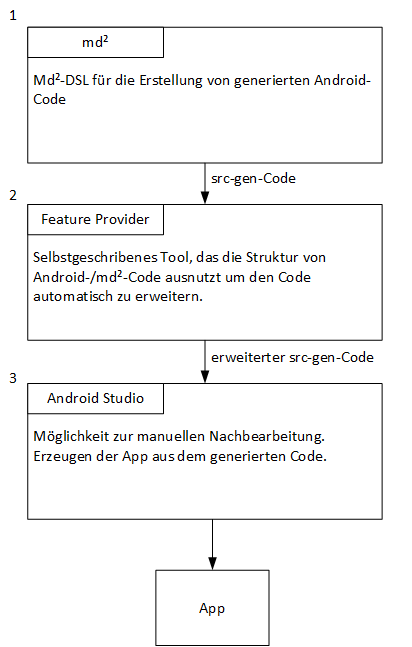
\epsfig{file = Abbildungen/Arbeitsschritte.png, width = 5.5cm}}
	\caption{Es werden die einzelnen Arbeitsschritte dargestellt. Die Zahlen geben die Reihenfolge der Schritte an. An den Pfeilen steht die Ausgabe des Vorg\"angerschritts, die als Eingabe des n\"achsten Schritts dient.}
	\label{fig:Arbeitsschritte}
\end{figure}

\noindent Der Code, der von $\text{MD}^2$ erzeugt wird, wird in einen Ordner mit dem Namen "src-gen" gespeichert. Auf diesem Code arbeitet der Feature Provider weiter. Das Ergebnis des Feature Providers wird in dem gleichen Ordner gespeichert. Nachdem der Code erweitert wurde kann er mit Android Studio ge\"offnet werden. Bei Bedarf k\"onnen manuelle Ver\"anderungen an dem Code vorgenommen werden. In Android Studio kann die App dann kompiliert und getestet werden.

\subsection{Feature Provider-Entwicklung}
Bei der Entwicklung des Feature Providers werden die Erkenntnisse der klassischen Programmierung ausgenutzt. Dabei werden allgemein g\"ultige Konzepte benutzt, sowie das Wechseln einer Activity mit Hilfe eines Intents. F\"ur die Umsetzung der Kommunikation mit einem REST-Service gibt es verschiedene Bibliotheken. Der Feature Provider benutzt ausschlie\ss{}lich die Bibliotheken, die bei der klassisch programmierten App benutzt wurden.\\
Zuerst wurde die Benutzeroberfl\"ache entwicklet, die es erm\"oglicht die entsprechenden Einstellungen auszuw\"ahlen. Besonders wichtig ist, die Auswahl des "src-gen"-Ordners, da der Absolute Pfad zu diesem Ordner auf jedem Ger\"at anders ist.\\
Danach wurde die Funktionalit\"at des Erzeugens der Features implementiert.\\
Zur Entwicklung der Funktionalit\"at des Feature Providers wurde in den von $\text{MD}^2$ erzeugten Code geschaut an welcher Stelle zus\"atzlicher Code eingef\"ugt werden muss, oder wo der Code durch anderen ersetzt werden muss. In der klassischen App wurde der Code gepr\"uft, wie die Funktionalit\"at umgesetzt wurde. Bei der Erstellung des Feature Providers wurden dann einige Klassen direkt \"ubernommen mit einigen Ver\"anderungen. Nach der Erzeugung einer neuen Funktion des Feature Providers wurden die in Abbildung \ref{fig:Arbeitsschritte} dargestellten Arbeitsschritte durchgef\"uhrt um zu testen, ob die App dann noch funktioniert und um zu sehen, dass das gewollte Feature hinzugef\"ugt wurde.
	\section{\uppercase{Werkzeuge zur Entwicklung}}
	
	\subsection{$\text{MD}^2$}
	$\text{MD}^2$-DSL ist eine dom\"anenspezifische Sprache (DSL), die entwickelt wurde um datengetriebene Business-Apps in textueller Form beschreiben zu k\"onnen \cite{DSLMD2_2013}.\\
	$\text{MD}^2$ ist ein akademischer Prototyp, der auch Anwendung in praktischen Projekten findet und dabei auch weiterentwickelt wird \cite{MDCP2015}.
	
	\subsection{Androidstudio}

	\subsection{FeatureProvider}
	

	\section{\uppercase{Entwicklung}}
\subsection{Schnittstellen}
Hier werden die Schnittstellen beschrieben, die mithilfe vom Restservice vom Server zur verf\"ugung stehen.
\begin{enumerate}
\item Operationen auf einen Nutzer
	\begin{itemize}
	\item Post (erstellung von einem Nutzer) \\
Hier ist die Erstellung von einem Nutzer m\"oglich. Wenn ein Nutzer unsere App. benutzen will, muss er erstmal sich registrieren lassen. Daf\"ur braucht man: \\
	- Ein Username \\
	- Ein Passwort \\
Antwort 200: Die Operation war erfolgreich\\ 
Antwort 400: Schlechte Anfrage, falls der Nutzer ung\"ultige oder schon vorhandene Parameter eintr\"agt.  

	\item Post (Nutzer im System einloggen) \\
Hier ist das Einloggen von einem Nutzer im System m\"oglich. Diese Funktionnalit\"at ist nur m\"oglich, wenn der Nutzer schon registriert ist. Daf\"ur braucht man: \\
	- Ein Username \\
	- Ein Passwort \\
Antwort 200: Die Operation war erfolgreich \\ 
Antwort 400: Schlechte Anfrage, falls der Nutzer ung\"ultige oder schon vorhandene Parameter eintr\"agt.  
	\item Delete (Meldet die aktuelle angemeldete Benutzersitzung ab)
Hier ist die Abmeldung von der Sitzung m\"oglich. Daf\"ur braucht man den Token vom Nutzer \\
Antwort 200: Die Operation war erfolgreich \\ 
Antwort 400: Schlechte Anfrage, falls der Nutzer ung\"ultige oder schon vorhandene Parameter eintr\"agt.  
	\end{itemize}

\item Operationen auf eine Datei
	\begin{itemize}
	\item Post (Hochladen von Dateien)
Hier ist das Hochladen von einer Datei m\"oglich. Daf\"ur braucht man: \\
	- Der Token \\
	- Der FolderId \\
	- Die Datei \\
Antwort 200: Die Operation war erfolgreich \\ 
Antwort 400: Schlechte Anfrage, Im Fall die Gr\"o{\ss}e der Datei gr\"o{\ss}er als 30Mb ist. \\
Antwort 403: Verboten \\
Antwort 404: Nicht gefunden
	\item Get (Herunterladen von Dateien)
Hier ist das herunterladen von einer Datei m\"oglich. Daf\"ur braucht man: \\
	- Der Token \\
	- Der FolderId (Id vom \"ubergeordneten Ordner) \\
	- Die DateiId (Id von der Datei) \\
Antwort 200: Die Operation war erfolgreich \\ 
Antwort 403: Verboten \\
Antwort 404: Nicht gefunden
	\item Put (Bearbeitung vom Dateiname)
Hier ist die Bearbeitung von einer Datei m\"oglich. Daf\"ur braucht man: \\
	- Der Token \\
	- Der FolderId (Id vom \"ubergeordneten Ordner) \\
	- Die DateiId (Id von der Datei) \\
	- Der Name von der Datei \\
Antwort 200: Die Operation war erfolgreich \\ 
Antwort 400: Schlechte Anfrage \\
Antwort 403: Verboten \\
Antwort 404: Nicht gefunden
	\item Delete (Löschen von einer Datei)
Hier ist das L\"oschen von einer Datei m\"oglich. Daf\"ur braucht man: \\
	- Der Token \\
	- Der FolderId (Id vom \"ubergeordneten Ordner) \\
	- Die DateiId (Id von der Datei) \\
Antwort 200: Die Operation war erfolgreich \\ 
Antwort 403: Verboten \\
Antwort 404: Nicht gefunden
	\end{itemize}

\item Operationen auf ein verzeichnis
	\begin{itemize}
	\item Get (Herunterladen von einem Ordner)
Hier ist das herunterladen von einem Ordner m\"oglich. Daf\"ur braucht man: \\
	- Der Token \\
	- Der FolderId (Id vom  Ordner) \\
Antwort 200: Die Operation war erfolgreich \\ 
Antwort 403: Verboten \\
Antwort 404: Nicht gefunden
	\item Post (Hochladen von einem Ordner) \\
Hier ist das Hochladen von einem Ordner m\"oglich. Daf\"ur braucht man: \\
	- Der Token \\
	- Der FolderId \\
	- Der Ordner\\
Antwort 200: Die Operation war erfolgreich \\ 
Antwort 400: Schlechte Anfrage, Im Fall die Gr\"o{\ss}e der Datei gr\"o{\ss}er als 30Mb ist. \\
Antwort 403: Verboten \\
Antwort 404: Nicht gefunden
	\item Put
	\item Delete
	\end{itemize}
\end{enumerate}
	\section{\uppercase{Zusammenfassung und Ausblick}}
\noindent Das Werkzeug $\text{MD}^2$ hat sich in der verwendeten Version als nicht so m\"achtig erwiesen, wie es gedacht war, weshalb nur ein geringer Anteil der App mit $\text{MD}^2$ umgesetzt werden konnte. Die Entwicklung eines Feature Providers, der auf dem von $\text{MD}^2$ erzeugten Code weiterarbeitet bot eine M\"oglichkeit das Erzeugen von Quellcode selber umzusetzen, auch wenn der Feature Provider ein sehr eingeschr\"anktes Werkzeug ist, das nur bei diesem Projekt eingesetzt werden kann. Die Umsetzung aller gew\"unschten Funktionen konnte nicht f\"ur die App realisiert werden, die mit $\text{MD}^2$ erzeugt wurde. Allerdings gibt es eine klassisch programmierte App, die den vollen Funktionsumfang bietet, die als Grundlage f\"ur \"Uberlegungen zur Erweiterung des Feature Providers dienen kann. Zuk\"unftig k\"onnten noch weitere Funktionen umgesetzt werden, der Feature Provider k\"onnte allgemeiner gemacht werden, sodass er f\"ur beliebige Anwendungen anwendbar ist.\\
Methoden der MDSD k\"onnen gut eingesetzt werden, um Android Apps zu generieren. Daf\"ur haben Android Apps entsprechende Strukturen, die sich in der Aufteilung der Code-Elemente wiederfinden. Als Beispiel daf\"ur seinen die Lebenszyklusmethoden genannt und die Aufteilung der View und Activity in verschiedenen Dateien.
	
	
	
	
	\bibliographystyle{apalike}
	\small
	\bibliography{example}
\end{document}